\documentclass[letterpaper,12pt]{article}

\usepackage{geometry, pslatex, fancyhdr, graphicx}
\usepackage{amsmath,amsthm,amssymb,scrextend}
\usepackage{multicol}
\usepackage{tabularx}
\usepackage[makeroom]{cancel}
\usepackage{color}
\geometry{ margin = 1.0in }

%%% TODO modify these variables as per your homework %%%
\def\homeworknum{3}
\def\myname{Harshit Jain}
\def\myuserid{hmj5262}
%%%%

\pagestyle{fancy}
\lhead{{\bf CMPSC 464 Spring 2024}}
\chead{{\bf Assignment~\homeworknum}}
\rhead{{\bf \today}}
\let\newproof\proof
\renewenvironment{proof}{\begin{addmargin}[1em]{0em}\begin{newproof}}{\end{newproof}\end{addmargin}\qed}

\newcounter{problemid}
\stepcounter{problemid}
\def\newproblem{\clearpage\newpage{\bf Problem~\arabic{problemid}\stepcounter{problemid}}\hfill\par}

\setlength\parindent{0em} 
\setlength\parskip{8pt}
\setlength{\fboxsep}{6pt}
 

\begin{document}

\framebox[\textwidth]{
	\parbox{0.96\textwidth}{
		\parbox{0.12\textwidth}{\bf Name:}\parbox{0.6\textwidth}{\myname}\\
		\parbox{0.12\textwidth}{\bf User ID:}\parbox{0.6\textwidth}{\myuserid}
	}
}

I collaborated with Yug Jarodiya.
%% your solutions %%%


% PROBLEM 1
\newproblem

The language consisting of strings of the form $a^{i} b^{j}$ where $i \neq j$ requires the grammar to capture the imbalance between the number of $a$'s and $b$'s.

We will re-write $i \neq j$ as $i < j$ or $i > j$.

L $= \{ a^{i} b^{j}$ ; $i < j$ or $i > j \}$

S $\rightarrow$ $A_{i < j}$ $\mid$ $A_{i > j}$ \\
$A_{i < j}$ $\rightarrow$ a$A_{i < j}$b $\mid$ bB \\
B $\rightarrow$ bB $\mid$ $\epsilon$ \\
$A_{i > j}$ $\rightarrow$ a$A_{i > j}$b $\mid$ aX \\
X $\rightarrow$ aX $\mid$ $\epsilon$

% PROBLEM 2
\newproblem
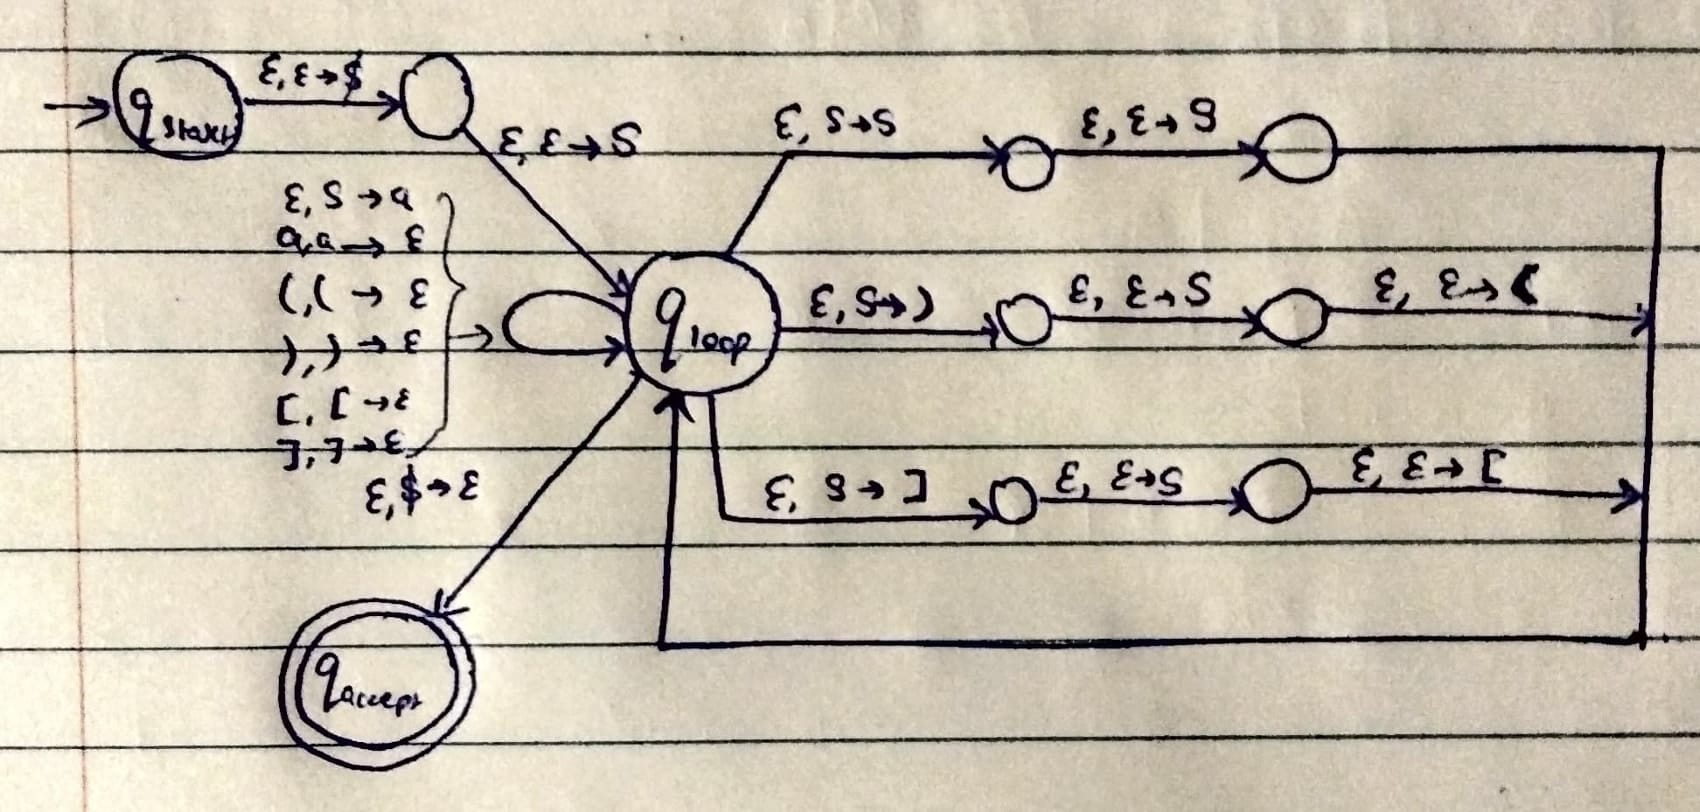
\includegraphics[scale = 0.25]{2}

% PROBLEM 3
\newproblem

A context free grammar (CFG) is in Chomsky Normal Form (CNF) if all production rules satisfy one of the following conditions:
\begin{itemize}
    \item A non-terminal generating a terminal (e.g.; X $\rightarrow$ x)
	\item A non-terminal generating two non-terminals (e.g.; X $\rightarrow$ YZ)
	\item Start symbol generating $\epsilon$. (e.g.; S $\rightarrow \epsilon$)
\end{itemize}

\textbf{Step 1:} As start symbol S appears on the RHS, we will create a new production rule S0 $\rightarrow$ S. Therefore, the grammar will become:

S0 $\rightarrow$ S \\
S $\rightarrow$ aSb $\mid$ c $\mid$ SS

\textbf{Step 2:} The grammar does not contain any null production.

\textbf{Step 3:} The rule S $\rightarrow$ aSb violates CNF because it has a unit production (a single terminal "a") on the right-hand side and rewrites to a non-terminal (S) followed by two symbols (a terminal "b"). 
After eliminating unit productions:

S0 $\rightarrow$ aSb $\mid$ c $\mid$ SS \\
S $\rightarrow$ aSb $\mid$ c $\mid$ SS

\textbf{Step 4:} In production rule S0 $\rightarrow$ aSb and S $\rightarrow$ aSb, RHS has more than two symbols, removing it from grammar yields:

S0 $\rightarrow$ XB $\mid$ c $\mid$ SS \\
S $\rightarrow$ XB $\mid$ c $\mid$ SS \\
X $\rightarrow$ aS \\
B $\rightarrow$ b

\textbf{Step 5:} After eliminating terminals from RHS since they exist with other terminals or non-terminals yields:

S0 $\rightarrow$ XB $\mid$ c $\mid$ SS \\
S $\rightarrow$ XB $\mid$ c $\mid$ SS \\
X $\rightarrow$ AS \\
A $\rightarrow$ a \\
B $\rightarrow$ b

% PROBLEM 4
\newproblem

Context-free grammar: S $\rightarrow$ SS $\mid$ aSb $\mid$ bSa $\mid$ $\epsilon$ 

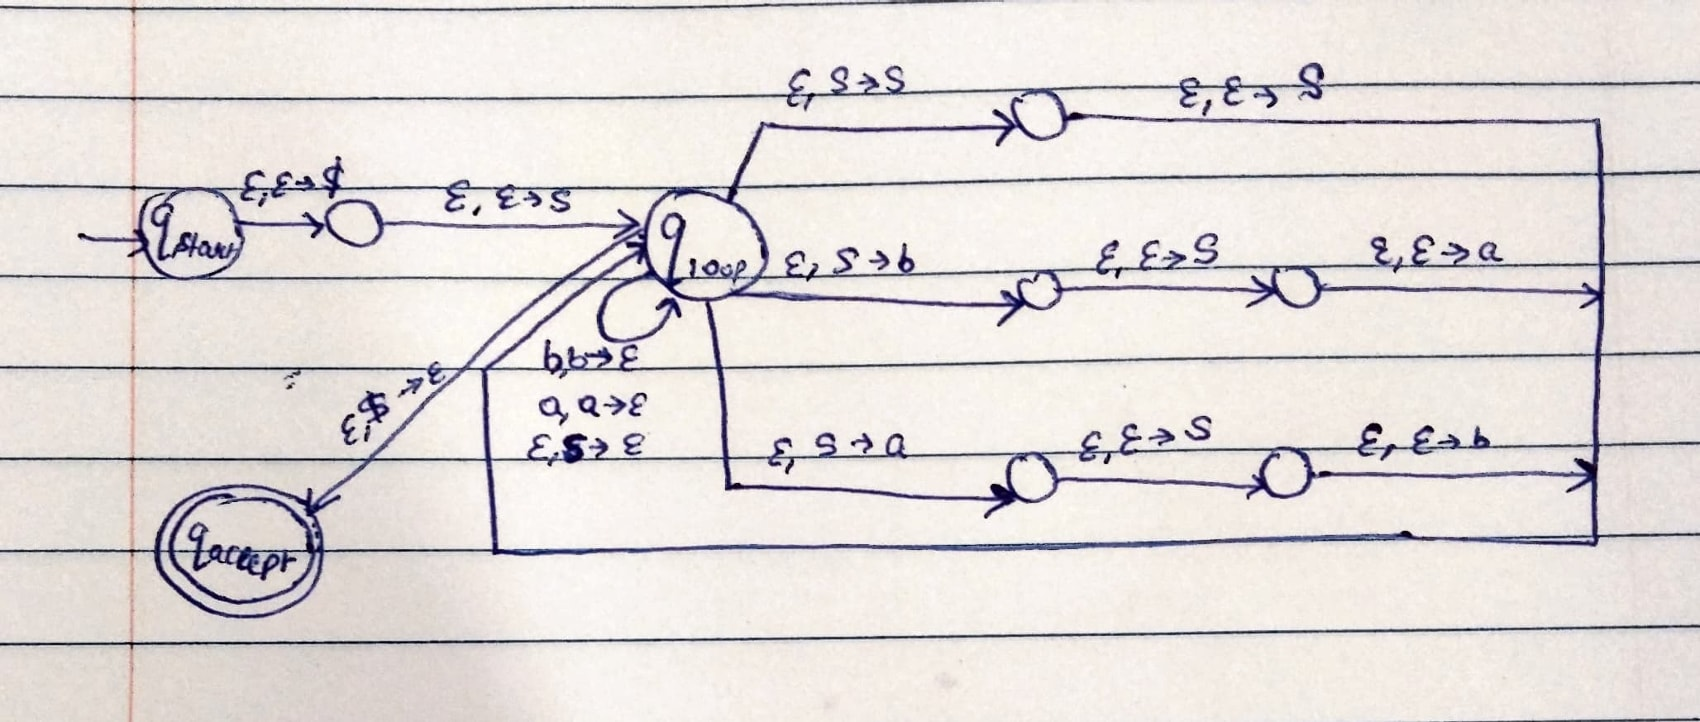
\includegraphics[scale = 0.25]{4}

\end{document}